% mnras_template.tex 
%
% LaTeX template for creating an MNRAS paper
%
% v3.2 released 20 July 2023
% (version numbers match those of mnras.cls)
%
% Copyright (C) Royal Astronomical Society 2015
% Authors:
% Keith T. Smith (Royal Astronomical Society)

%%%%%%%%%%%%%%%%%%%%%%%%%%%%%%%%%%%%%%%%%%%%%%%%%%
% Basic setup. Most papers should leave these options alone.
\documentclass[fleqn,usenatbib]{mnras}

% MNRAS is set in Times font. If you don't have this installed (most LaTeX
% installations will be fine) or prefer the old Computer Modern fonts, comment
% out the following line
\usepackage{newtxtext,newtxmath}
% Depending on your LaTeX fonts installation, you might get better results with one of these:
%\usepackage{mathptmx}
%\usepackage{txfonts}

% Use vector fonts, so it zooms properly in on-screen viewing software
% Don't change these lines unless you know what you are doing
\usepackage[T1]{fontenc}

% Allow "Thomas van Noord" and "Simon de Laguarde" and alike to be sorted by "N" and "L" etc. in the bibliography.
% Write the name in the bibliography as "\VAN{Noord}{Van}{van} Noord, Thomas"
\DeclareRobustCommand{\VAN}[3]{#2}
\let\VANthebibliography\thebibliography
\def\thebibliography{\DeclareRobustCommand{\VAN}[3]{##3}\VANthebibliography}


%%%%% AUTHORS - PLACE YOUR OWN PACKAGES HERE %%%%%

% Only include extra packages if you really need them. Avoid using amssymb if newtxmath is enabled, as these packages can cause conflicts. newtxmatch covers the same math symbols while producing a consistent Times New Roman font. Common packages are:
\usepackage{graphicx}	% Including figure files
\usepackage{amsmath}	% Advanced maths commands
\usepackage{lmodern}
\usepackage{anyfontsize}

%%%%%%%%%%%%%%%%%%%%%%%%%%%%%%%%%%%%%%%%%%%%%%%%%%

%%%%% AUTHORS - PLACE YOUR OWN COMMANDS HERE %%%%%

% Please keep new commands to a minimum, and use \newcommand not \def to avoid
% overwriting existing commands. Example:
%\newcommand{\pcm}{\,cm$^{-2}$}	% per cm-squared

\graphicspath{{images/}}

%%%%%%%%%%%%%%%%%%%%%%%%%%%%%%%%%%%%%%%%%%%%%%%%%%


%%%%%%%%%%%%%%%%%%% TITLE PAGE %%%%%%%%%%%%%%%%%%%

% Title of the paper, and the short title which is used in the headers.
% Keep the title short and informative.
\title[Short title, max. 45 characters]{Simple models to describe the star formation rate bimodality in galaxies at low redshift}

% The list of authors, and the short list which is used in the headers.
% If you need two or more lines of authors, add an extra line using \newauthor
\author[M. Bianchi]{
Marco Bianchi
\\
% List of institutions
University of Milano-Bicocca, Physics Department, Astrophysics and Space Physics master degree\\
Laboratory of Data Analysis 2023-2024, group 5: M. Bellotti, M. Bianchi, L. Carbone, and F. Leto Di Priolo\\
}

% Enter the current year, for the copyright statements etc.
\pubyear{2024}

% Don't change these lines
\begin{document}
\label{firstpage}
\pagerange{\pageref{firstpage}--\pageref{lastpage}}
\maketitle

% Abstract of the paper
\begin{abstract}
Galaxies at low redshift ($z<0.08$ for the data used here) display a bimodality in their specific Star Formation Rate (sSFR). This phenomenon is related to several factors, including (1) the accretion processes that drive galaxy growth, (2) the feedback processes that eject gas from galaxies, and (3) the interactions between galaxies and their surrounding environment. These processes are strongly influenced by key physical properties of galaxies, such as gas mass, stellar mass, and age. Therefore, it is possible to build models that describe the time evolution of sSFR based on these simple quantities. \\
We developed two very simple analytical models, based on strong assumptions, and applied them to a subset of the Sloan Digital Sky Survey (SDSS) dataset. Our findings indicate that young, actively star-forming galaxies can be described by an open-box model, while old, passive galaxies are better represented by a closed-box model, which does not exchange gas with the surrounding halo. We also relaxed some assumptions, such as redshift-independent gas accretion, by numerically integrating the differential equation of the open-box model over infinitesimal time steps, obtaining similar results.
\bigskip
\end{abstract} 
%%%%%%%%%%%%%%%%%%%%%%%%%%%%%%%%%%%%%%%%%%%%%%%%%%




%%%%%%%%%%%%%%%%% BODY OF PAPER %%%%%%%%%%%%%%%%%%

\section{Introduction}\label{sec:introduction}
What are the physical processes that determine the quenching of the sSFR for a fraction of the more massive galaxies? 
Is the development of such processes related to the age of the galaxy?

All papers should start with an Introduction section, which sets the work
in context, cites relevant earlier studies in the field by \citet{Kennicutt_1998},
and describes the problem the authors aim to solve \citep[e.g.][]{Dave_2011}.
Multiple citations can be joined in a simple way like \citet{KKennicutt_1998,Moster_2012}.

\begin{figure}
	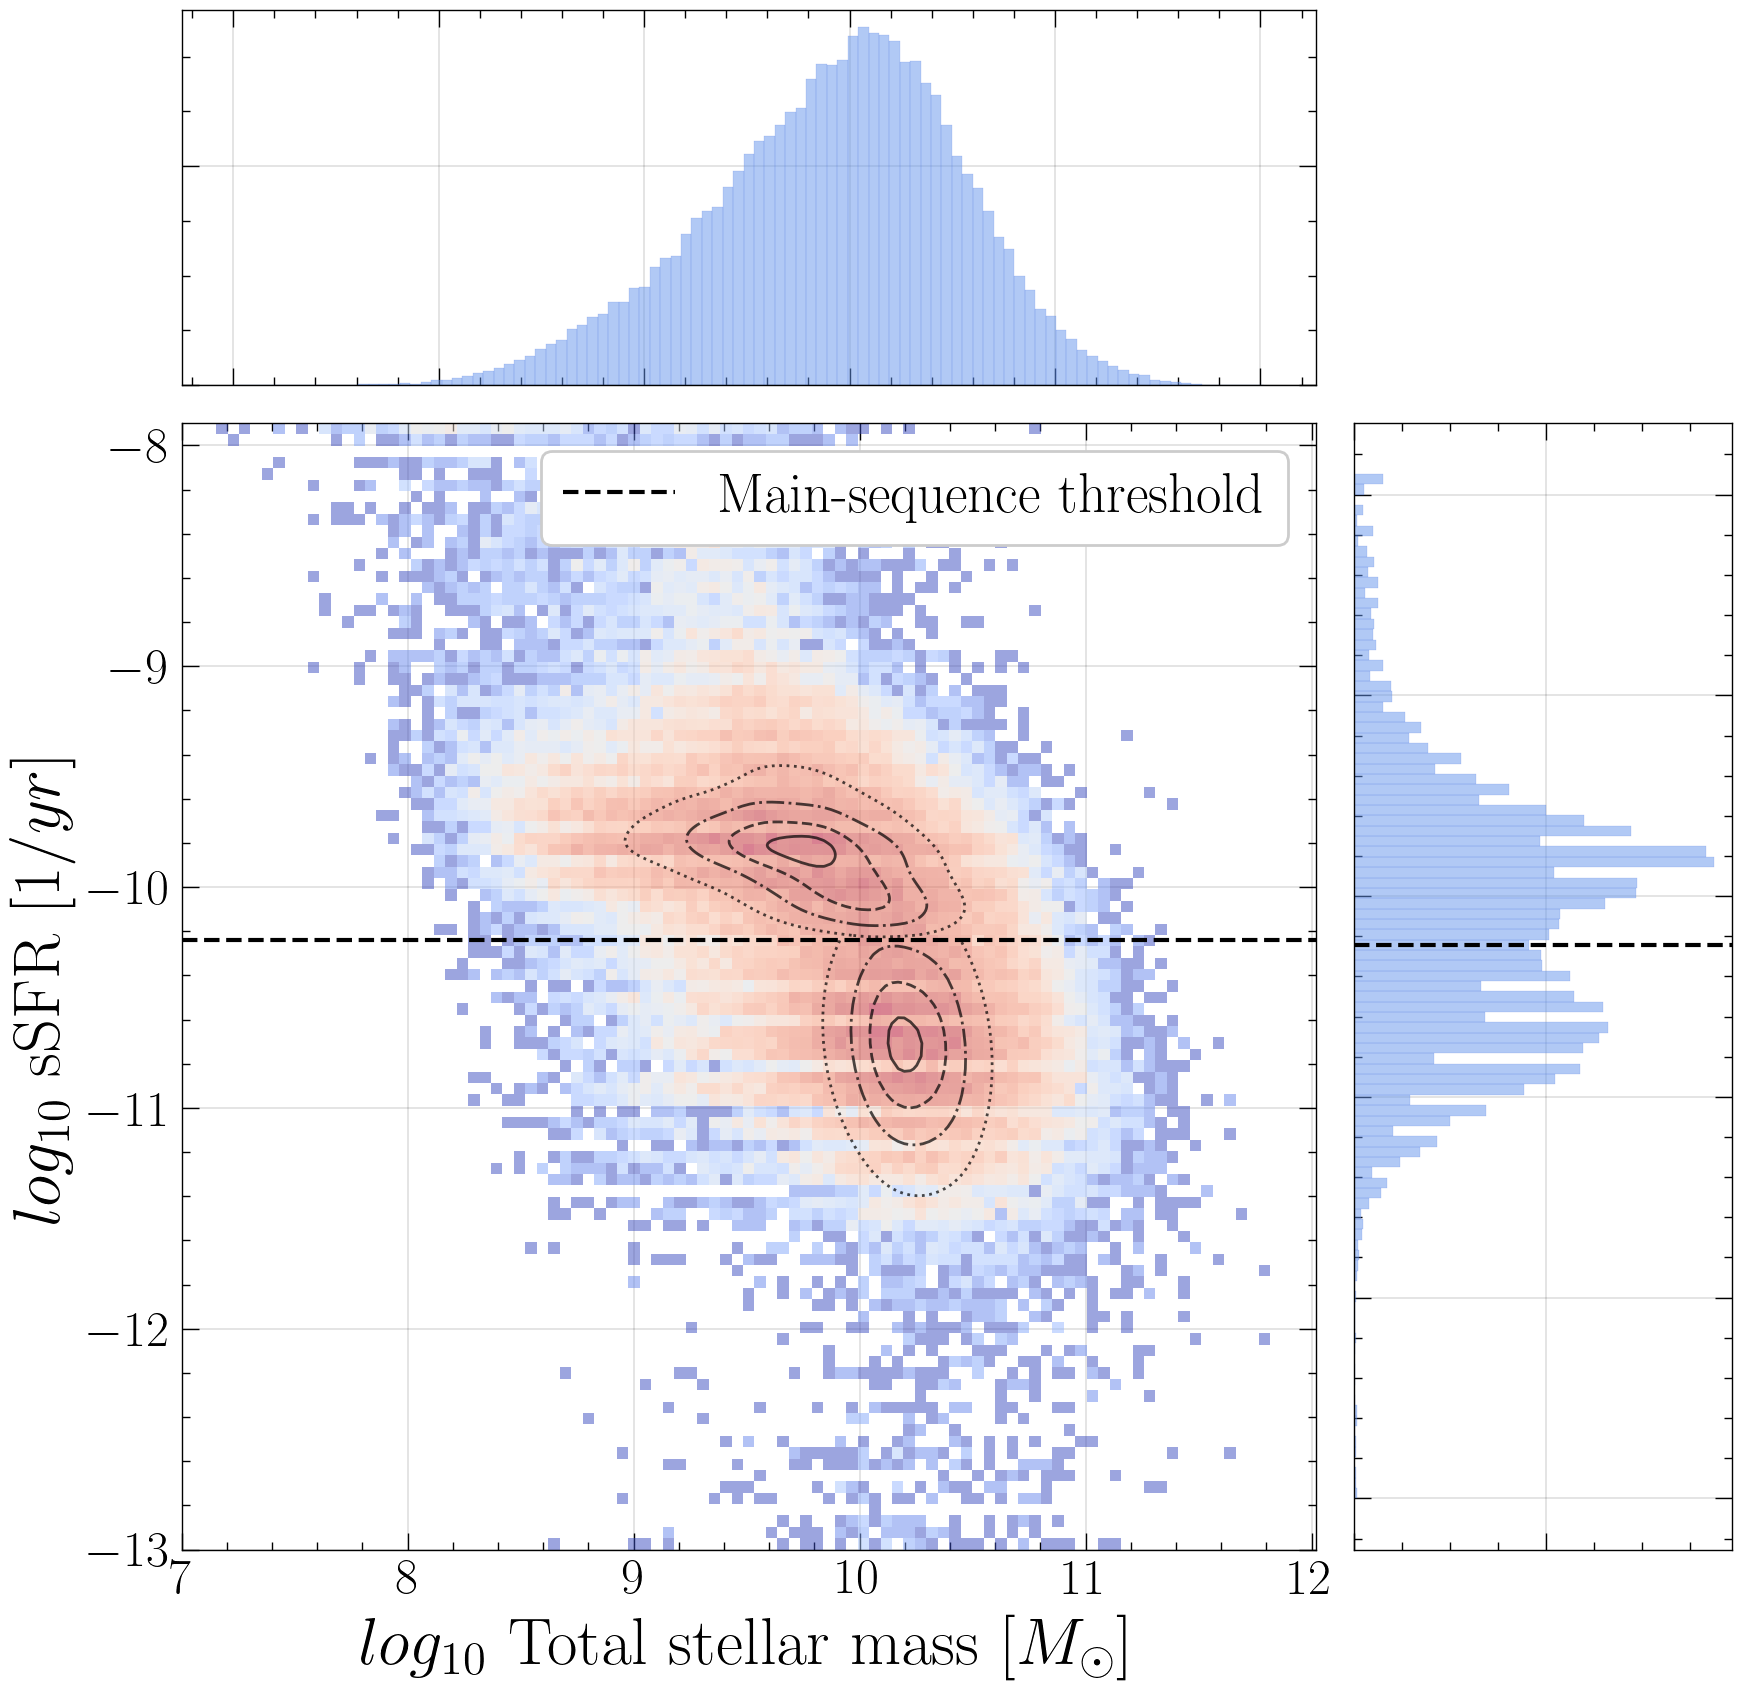
\includegraphics[width=\columnwidth]{mass_sSFR.png}
    \caption{This is an example figure. Captions appear below each figure.
	Give enough detail for the reader to understand what they're looking at,
	but leave detailed discussion to the main body of the text.}
    \label{fig:mass_sSFR}
\end{figure}



\section{Methods}\label{sec:methods}

\begin{equation}
    x=\frac{-b\pm\sqrt{b^2-4ac}}{2a}.
	\label{eq:quadratic}
\end{equation}

Refer back to them as e.g. equation~(\ref{eq:quadratic}).

Figures are referred to as e.g. Fig.~\ref{fig:mass_sSFR}



\section{Results}\label{sec:results}



\section{Discussion}\label{sec:discussion}



\section{Summary}\label{sec:summary}

%%%%%%%%%%%%%%%%%%%%%%%%%%%%%%%%%%%%%%%%%%%%%%%%%%




%%%%%%%%%%%%%%%%%%%% REFERENCES %%%%%%%%%%%%%%%%%%
% The best way to enter references is to use BibTeX:
\bibliographystyle{mnras}
\bibliography{bibliography} 
%%%%%%%%%%%%%%%%%%%%%%%%%%%%%%%%%%%%%%%%%%%%%%%%%%




% Don't change these lines
\label{lastpage}
\end{document}

% End of mnras_template.tex
